
Let us consider the following one-dimensional grid: 
\begin{center}
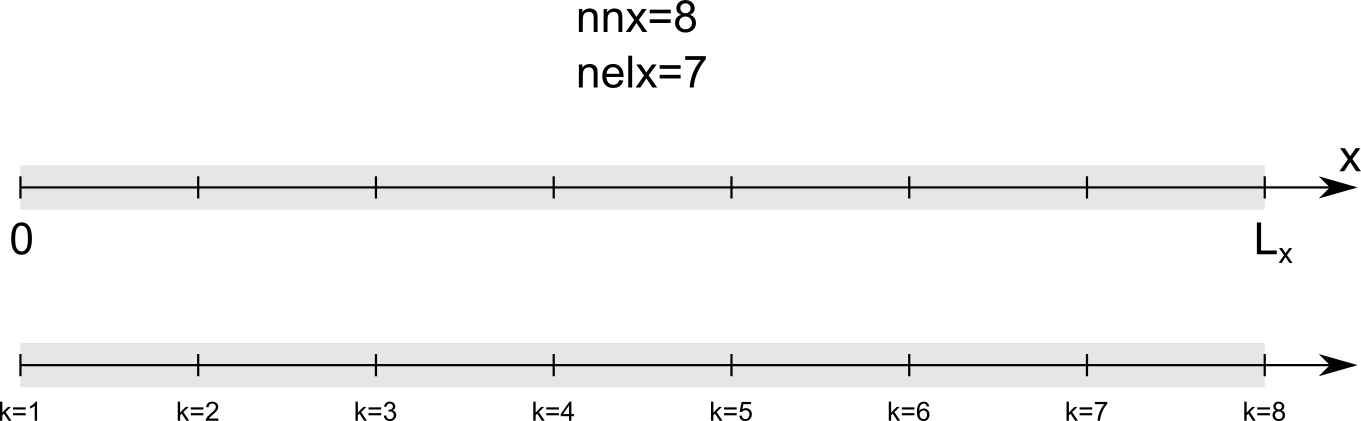
\includegraphics[width=10cm]{images/oneD/domain}
\end{center}
Its spans the domain $\Omega$ of length $L_x$. 
It is discretised by means of 
$nnx$ nodes and $nelx=nnx-1$ elements.
Zooming in on element which is bounded by two nodes $k$ and $k+1$,
its size (also sometimes called diameter) is $h_x=x_{k+1}-x_k$, 
and the temperature field we wish to compute is located on those 
nodes so that they are logically called $T_k$ and $T_{k+1}$:

\begin{center}
\includegraphics[width=8cm]{images/oneD/el1D}
\end{center}

We focus here on the 1D diffusion equation (no advection, no heat sources):
\begin{equation}
\rho C_p \frac{\partial T}{\partial t} 
= \frac{\partial }{\partial x} \left( k \frac{\partial T}{\partial x}  \right)
\end{equation}
This is the {\color{olive}strong form} of the ODE to solve.
I can multiply this equation by a function\footnote{This function should be well-behaved with special properties, but we here assume it is a polynomial function.} $f(x)$ and integrate it over $\Omega$:
\begin{equation}
\int_{\Omega} f(x)  \rho C_p\frac{\partial T}{\partial t} dx
=
\int_{\Omega} f(x) \frac{\partial }{\partial x} \left( k \frac{\partial T}{\partial x}  \right) dx
\end{equation}
Looking at the right hand side, it is of the form $\int u v'$ so that I naturally 
integrate it by parts:
\begin{equation}
\int_{\Omega} f(x) \frac{\partial }{\partial x} 
\left( k \frac{\partial T}{\partial x}  \right) dx
=
\left[
f(x) k \frac{\partial T}{\partial x}
\right]_{\partial \Omega}
-
\int_{\Omega} \frac{\partial f}{\partial x}  k \frac{\partial T}{\partial x}  dx
\end{equation}
Assuming there is no heat flux prescribed on the boundary (i.e. $q_x= - k \partial T/\partial x = 0$ ),
\todo[inline]{NOT happy with this statement!!} then:
\begin{equation}
\int_{\Omega} f(x) \frac{\partial }{\partial x} \left( k \frac{\partial T}{\partial x}  \right) dx
=
- \int_{\Omega} \frac{\partial f}{\partial x}  k \frac{\partial T}{\partial x}  dx
\end{equation}
We then obtain the {\color{olive}weak form} of the diffusion equation in 1D:
\begin{equation}
\boxed{
\int_{\Omega} f(x) \rho C_p \frac{\partial T}{\partial t} dx
+
\int_{\Omega} \frac{\partial f}{\partial x}  k \frac{\partial T}{\partial x}  dx = 0
}
\end{equation}
We then use the additive property of the integral 
$\int_\Omega \dots = \sum_{elts} \int_{\Omega_e} \dots$
so that 
\begin{equation}
\sum_{elts} \left(     
\underbrace{ \int_{\Omega_e} f(x) \rho C_p   \frac{\partial T}{\partial t} dx }_{{\Lambda}_f^e}
+
\underbrace{\int_{\Omega_e} \frac{\partial f}{\partial x}  k \frac{\partial T}{\partial x}  dx}_{{\Upsilon}_f^e}      \right) = 0  
\end{equation}

In order to compute these integrals (analytically or by means of a numerical quadrature), 
we will need to evaluate $T$ inside the element. However, inside the element, 
the temperature is not known: all we have is the temperature at the nodes. 
For $x\in [x_k,x_{k+1}]$ we need to come up with a way to compute the temperature at this location. 
It makes sense to think that $T(x)$ will then be a function of the temperature at the nodes, 
i.e. $T(x) = \alpha T_k + \beta T_{k+1}$ where $\alpha$ and $\beta$ are coefficients. 
One over-simplified approach would be to assign $T(x)=(T_k + T_{k+1})/2$ but this would make the
temperature discontinuous from element to element. 
The rather logical solution to this problem is a linear temperature field between $T_k$
and $T_{k+1}$: 

\begin{eqnarray}
T(x) 
%&=& N_{k}(x) T_k + N_{k+1}(x) T_{k+1}  \nn\\
&=& \underbrace{\frac{x_{k+1}-x}{h_x}}_{N_k^\theta(x)} T_k 
+ 
\underbrace{\frac{x-x_k}{h_x}}_{N_{k+1}^\theta(x)} T_{k+1} \nn
\end{eqnarray}
where $N_k^\theta(x)$ is the (temperature) shape function associated to node $k$ and 
$N_{k+1}^\theta(x)$ is the shape function associated to node $k+1$.

Rather reassuringly, we have:
\begin{itemize}
\item $x=x_k$ yields $T(x)=T_k$
\item $x=x_{k+1}$ yields $T(x)=T_{k+1}$
\item $x=(x_k+x_{k+1})/2$ yields $T(x)=(T_k+T_{k+1})/2$
\end{itemize}
In what follows we abbreviate $\partial T/\partial x$ by $\dot{T}$.
Let us compute ${\Lambda}_f^e$ and ${\Upsilon}_f^e$ separately.
\begin{eqnarray}
{\Lambda}_f^e 
&=&\int_{x_k}^{x_{k+1}} f(x) \rho C_p \dot T(x) dx \nn\\
&=& \int_{x_k}^{x_{k+1}} f(x) \rho C_p \;\;  [ N_{k}^\theta(x) \dot{T}_k + N_{k+1}^\theta(x) \dot{T}_{k+1} ] \;\; dx  \nn\\
&=& \int_{x_k}^{x_{k+1}} f(x) \rho C_p N_{k}^\theta(x) \dot{T}_k  dx  
+ \int_{x_k}^{x_{k+1}} f(x) \rho C_p N_{k+1}^\theta(x) \dot{T}_{k+1}   dx \nn\\
&=&  \left( \int_{x_k}^{x_{k+1}} f(x) \rho C_p  N_{k}^\theta(x) dx \right) \dot{T}_k  
+ \left( \int_{x_k}^{x_{k+1}} f(x) \rho C_p N_{k+1}^\theta(x) dx \right)  \dot{T}_{k+1}  \nn
\end{eqnarray}
Taking $f(x)=N_k^\theta(x)$ and omitting '$(x)$' in the rhs:
\[
{\Lambda}_{N_k^\theta}^e=
%\int_{x_k}^{x_{k+1}} {\color{blue}f}(x) \rho C_p \dot{\color{blue}T}(x) dx
\left( \int_{x_k}^{x_{k+1}} \rho C_p  N_k^\theta N_{k}^\theta dx \right) \dot{T}_k  
+ \left( \int_{x_k}^{x_{k+1}} \rho C_p N_k^\theta N_{k+1}^\theta dx \right)  \dot{T}_{k+1} 
\]
Taking $f(x)=N_{k+1}^\theta(x)$ and omitting '$(x)$' in the rhs:
\[
{\Lambda}_{N_{k+1}^\theta}^e
%\int_{x_k}^{x_{k+1}} {\color{blue}f}(x) \dot{\color{blue}T}(x) dx
=  \left( \int_{x_k}^{x_{k+1}} \rho C_p N_{k+1}^\theta N_{k}^\theta dx \right) \dot{T}_k  
+ \left( \int_{x_k}^{x_{k+1}}  \rho C_p  N_{k+1}^\theta N_{k+1}^\theta dx \right)  \dot{T}_{k+1} 
\]
We can rearrange these last two equations as follows:
\[
\left(
\begin{array}{c}
{\Lambda}_{N_k^\theta}^e  \\ \\ {\Lambda}_{N_{k+1}^\theta}^e
\end{array}
\right)
=
\left(
\begin{array}{cc}
\int_{x_k}^{x_{k+1}} N_k^\theta     \rho C_p N_{k}^\theta dx  &  \int_{x_k}^{x_{k+1}} N_k^\theta  \rho C_p N_{k+1}^\theta dx \\ \\
\int_{x_k}^{x_{k+1}} N_{k+1}^\theta \rho C_p N_{k}^\theta dx  &  \int_{x_k}^{x_{k+1}} N_{k+1}^\theta \rho C_p N_{k+1}^\theta dx 
\end{array}
\right)
\cdot
\left(
\begin{array}{c}
\dot{T}_k \\ \\
\dot{T}_{k+1}
\end{array}
\right)
\]
and we can take the integrals outside of the matrix:
\[
\left(
\begin{array}{c}
{\Lambda}_{N_k^\theta}^e \\ \\ {\Lambda}_{N_{k+1}^\theta}^e
\end{array}
\right)
=
\left[
\int_{x_k}^{x_{k+1}}
\rho C_p
\left(
\begin{array}{cc}
N_k^\theta N_{k}^\theta     &  N_k^\theta N_{k+1}^\theta  \\ \\
N_{k+1}^\theta N_{k}^\theta &  N_{k+1}^\theta N_{k+1}^\theta 
\end{array}
\right)
dx
\right]
\cdot
\left(
\begin{array}{c}
\dot{T}_k \\ \\ 
\dot{T}_{k+1}
\end{array}
\right)
\]
Finally, we can define the vectors 
\[
{\vec N}^T = 
\left(
\begin{array}{c}
N_k^\theta(x)  \\ \\  N_{k+1}^\theta (x)
\end{array}
\right)
\]
and 
\[
{\vec T}^e = 
\left(
\begin{array}{c}
T_k \\ \\ T_{k+1}
\end{array}
\right)
\quad
\quad
\quad
\quad
\quad
\dot{\vec T}^e = 
\left(
\begin{array}{c}
\dot{T}_k \\ \\ \dot{T}_{k+1}
\end{array}
\right)
\]
so that 
\[
\left(
\begin{array}{c}
{\Lambda}_{N_k^\theta}^e \\  \\ {\Lambda}_{N_{k+1}^\theta}^e
\end{array}
\right)
=
\left( \int_{x_k}^{x_{k+1}}   {\vec N}^T \rho C_p  {\vec N} dx  \right) \cdot \dot{\vec T}^e
\]

Back to the diffusion term:

\begin{eqnarray}
{\Upsilon}_f^e &=&
\int_{x_k}^{x^{k+1}} \frac{\partial f}{\partial x} k \frac{\partial T}{\partial x} dx \nn\\
&=&
\int_{x_k}^{x^{k+1}} \frac{\partial f}{\partial x} k \frac{\partial  (N_{k}^\theta(x) T_k + N_{k+1}^\theta(x) T_{k+1} ) }{\partial x} dx  \nn\\
%&=&
%\int_{x_k}^{x^{k+1}} \left( \frac{\partial {\color{blue}f}}{\partial x}  \frac{\partial  {\color{blue}N}_{k} } {\partial x}  T_k 
%+ \frac{\partial {\color{blue}f}}{\partial x}  \frac{\partial  {\color{blue}N}_{k+1} } {\partial x}  T_{k+1} \right)  dx \nn\\
&=&
\left( \int_{x_k}^{x^{k+1}} \frac{\partial f}{\partial x}  k \frac{\partial  N_{k}^\theta } {\partial x}  dx \right)  T_k 
+ \left( \int_{x_k}^{x^{k+1}} \frac{\partial f}{\partial x}  k \frac{\partial  N_{k+1}^\theta } {\partial x} dx \right) T_{k+1}  \nn
\end{eqnarray}
Taking $f(x)=N_k^\theta(x)$ 
\[
{\Upsilon}_{N_k^\theta}^e=
%\int_{x_k}^{x^{k+1}} \frac{\partial {\color{blue}f}}{\partial x} \frac{\partial {\color{blue}T}}{\partial x} dx
\left( \int_{x_k}^{x^{k+1}} k\frac{\partial N_k^\theta}{\partial x}  \frac{\partial  N_{k}^\theta } {\partial x}  dx \right)  T_k 
+ \left( \int_{x_k}^{x^{k+1}} k \frac{\partial N_k^\theta}{\partial x}  \frac{\partial  N_{k+1}^\theta } {\partial x} dx \right) T_{k+1}  \nn
\]
Taking $f(x)=N_{k+1}^\theta(x)$ 
\[
{\Upsilon}_{N_{k+1}^\theta}^e=
%\int_{x_k}^{x^{k+1}} \frac{\partial {\color{blue}f}}{\partial x} \frac{\partial {\color{blue}T}}{\partial x} dx
%=
\left( \int_{x_k}^{x^{k+1}} k\frac{\partial N_{k+1}^\theta}{\partial x}  \frac{\partial  N_{k}^\theta } {\partial x}  dx \right)  T_k 
+ \left( \int_{x_k}^{x^{k+1}}  k\frac{\partial N_{k+1}^\theta}{\partial x}  \frac{\partial  N_{k+1}^\theta } {\partial x} dx \right) T_{k+1}  \nn
\]


\[
\left(
\begin{array}{cc}
 {\Upsilon}_{N_k^\theta}^e \\ \\ {\Upsilon}_{N_{k+1}^\theta}^e
\end{array}
\right)
=
\left(
\begin{array}{cc}
\int_{x_k}^{x^{k+1}} \frac{\partial N_k^\theta}{\partial x} k \frac{\partial  N_{k}^\theta } {\partial x}  dx & 
\int_{x_k}^{x^{k+1}} \frac{\partial N_k^\theta}{\partial x} k \frac{\partial  N_{k+1}^\theta } {\partial x} dx 
\\ \\
\int_{x_k}^{x^{k+1}} \frac{\partial N_{k+1}^\theta}{\partial x} k \frac{\partial  N_{k}^\theta } {\partial x}  dx & 
\int_{x_k}^{x^{k+1}} \frac{\partial N_{k+1}^\theta}{\partial x} k \frac{\partial  N_{k+1}^\theta } {\partial x} dx 
\end{array}
\right)
\cdot
\left(
\begin{array}{c}
T_k \\ \\ T_{k+1}
\end{array}
\right)
\]

or,
\[
\left(
\begin{array}{cc}
 {\Upsilon}_{N_k^\theta}^e \\ \\ {\Upsilon}_{N_{k+1}^\theta}^e
\end{array}
\right)
=
\left[
\int_{x_k}^{x^{k+1}}
k
\left(
\begin{array}{cc}
\frac{\partial N_k^\theta}{\partial x}  \frac{\partial  N_{k}^\theta } {\partial x}   & 
\frac{\partial N_k^\theta}{\partial x}  \frac{\partial  N_{k+1}^\theta } {\partial x}  
\\ \\
\frac{\partial N_{k+1}^\theta}{\partial x}  \frac{\partial  N_{k}^\theta } {\partial x}   & 
\frac{\partial N_{k+1}^\theta}{\partial x}  \frac{\partial  N_{k+1}^\theta } {\partial x}  
\end{array}
\right)
dx
\right]
\cdot
\left(
\begin{array}{c}
T_k \\ \\ T_{k+1}
\end{array}
\right)
\]
Finally, we can define the vector 
\[
{\vec B}^T=
\left(
\begin{array}{cc}
 \frac{\partial N_k^\theta}{\partial x}   \\ \\
 \frac{\partial N_{k+1}^\theta}{\partial x}
\end{array}
\right)
\]
so that 
\[
\left(
\begin{array}{cc}
 {\Upsilon}_{N_k^\theta}^e \\ \\ {\Upsilon}_{N_{k+1}^\theta}^e
\end{array}
\right)
=
\left( \int_{x_k}^{x_{k+1}}   {\vec B}^T k {\vec B} dx  \right) \cdot {\vec T}^e
\]

The weak form discretised over 1 element becomes
\[
\underbrace{\left( \int_{x_k}^{x_{k+1}}   {\vec N}^T \rho C_p {\vec N} dx  \right) }_{\bm M^e} \cdot \dot{\vec T}^e
+
\underbrace{\left( \int_{x_k}^{x_{k+1}}   {\vec B}^T k {\vec B} dx  \right)}_{{\bm K}_d^e} \cdot {\vec T}^e
=0
\]
or,
\[
\boxed{
{\bm M}^e \cdot \dot{\vec T}^e + {\bm K}_d^e \cdot {\vec T}^e = 0
}
\]
or,
\[
\boxed{
{\bm M}^e \cdot \frac{\partial {\vec T}^e}{\partial t} + {\bm K}_d^e \cdot {\vec T}^e = 0
}
\]

Using a backward first order in time discretisation for the time derivative:
\[
\dot{\vec T}= \frac{\partial {\vec T}}{\partial t} = \frac{{\vec T}^{new}-{\vec T}^{old}}{\delta t}
\]
we get
\[
{\bm M}^e \cdot \frac{{\vec T}^{new}-{\vec T}^{old}}{\delta t} + {\bm K}_d^e \cdot {\vec T}^{new} = 0
\]
or, 
\[
\boxed{
( {\bm M}^e +  {\bm K}_d^e  \delta t ) \cdot {\vec T}^{new} =  {\bm M}^e \cdot  {\vec T}^{old}
}
\]
with 
\[
{\bm M}^e=  \int_{x_k}^{x_{k+1}}   {\vec N}^T \rho C_p {\vec N} dx  
\quad\quad\quad
{\bm K}_d^e =
 \int_{x_k}^{x_{k+1}}   {\vec B}^T k {\vec B} dx 
\]

Let us compute ${\bm M}$ for an element:
\[
{\bm M}^e=  \int_{x_k}^{x_{k+1}}   {\vec N}^T \rho C_p {\vec N} dx  
\]
with 
\[
{\vec N}^T = 
\left(
\begin{array}{c}
N_k(x)  \\ \\  N_{k+1}(x)
\end{array}
\right)
=
\left(
\begin{array}{c}
\frac{x_{k+1}-x}{h_x}   \\ \\
\frac{x-x_k}{h_x} 
\end{array}
\right)
\]
Then 
\[
{\bm M}^e
=
\left(
\begin{array}{cc}
M_{11} & M_{12} \\
M_{21} & M_{22} 
\end{array}
\right)
=
\left(
\begin{array}{cc}
\int_{x_k}^{x_{k+1}} \rho C_p N_k^\theta N_{k}^\theta dx   &  \int_{x_k}^{x_{k+1}} \rho C_p N_k^\theta N_{k+1}^\theta dx \\ \\
\int_{x_k}^{x_{k+1}} \rho C_p N_{k+1}^\theta N_{k}^\theta dx  &  \int_{x_k}^{x_{k+1}} \rho C_p N_{k+1}^\theta N_{k+1}^\theta dx 
\end{array}
\right)
\]
I only need to compute 3 integrals since $M_{12}=M_{21}$.
Let us start with $M_{11}$:
\[
M_{11}=\int_{x_k}^{x_{k+1}} \rho C_p N_k^\theta(x) N_{k}^\theta(x) dx
=   
\int_{x_k}^{x_{k+1}} \rho C_p 
\frac{x_{k+1}-x}{h_x}  
\frac{x_{k+1}-x}{h_x}  
dx
\]
It is then customary to carry out the change of variable $x \rightarrow r$ where 
$r \in [-1:1]$ as shown hereunder:
\begin{center}
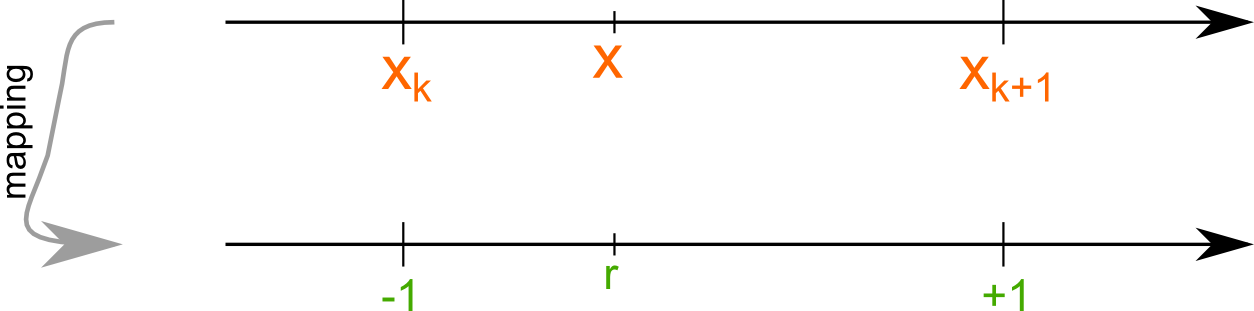
\includegraphics[width=8cm]{images/oneD/el1D_mapping}
\end{center}
The relationships between $x$ and $r$ are:
\[
r=\frac{2}{h_x}(x-x_k)-1
\quad\quad\quad
x=\frac{h_x}{2}(1+r)+x_k
\]

In what follows we assume for simplicity that $\rho$ and $C_p$ are constant within each element.
\[
M_{11}=
\rho C_p
\int_{\tiny x_k}^{x_{k+1}} 
\frac{x_{k+1}-x}{h_x}  
\frac{x_{k+1}-x}{h_x}  
dx
%=  \rho C_p \int_{-1}^{+1} \frac{1}{2}(1-r) \frac{1}{2}(1-r)  \frac{h_x}{2} dr  = \frac{h_x}{3} \rho C_p \nn
=  \frac{\rho C_p h_x}{8} \int_{-1}^{+1} (1-r) (1-r)  dr  = \frac{h_x}{3} \rho C_p
\]
Similarly we arrive at 
\begin{eqnarray}
M_{12}
%\rho C_p \int_{x_k}^{x_{k+1}}  {\color{blue}N}_k(x) {\color{blue}N}_{k+1}(x) dx
=\rho C_p 
\int_{x_k}^{x_{k+1}} 
\frac{x_{k+1}-x}{h_x}  
\frac{x-x_k}{h_x}  
dx
=
\frac{\rho C_p  h_x}{8} 
\int_{-1}^{+1} (1-r) (1+r)dr
= \frac{h_x}{6} \rho C_p \nn
\end{eqnarray}
and 
\[
M_{22}
%=\rho C_p \int_{x_k}^{x_{k+1}} {\color{blue}N}_{k+1}(x) {\color{blue}N}_{k+1}(x) dx
=
\rho C_p 
\int_{x_k}^{x_{k+1}} 
\frac{x-x_k}{h_x}  
\frac{x-x_k}{h_x}  
dx
=
\frac{\rho C_p  h_x}{8} 
\int_{-1}^{+1} (1+r) (1+r)dr
= \frac{h_x}{3} \rho C_p 
\]
Finally 
\[
\boxed{
{\bm M}^e= \frac{h_x}{3} \rho C_p  
\left(
\begin{array}{cc}
1  & 1/2 \\
1/2 & 1
\end{array}
\right)
}
\]

In the new coordinate system, the {\color{olive}shape functions} 
\[
N_k^\theta(x) = \frac{x_{k+1}-x}{h_x} 
\quad
\quad
\quad
N_{k+1}^\theta(x) = \frac{x-x_k}{h_x} 
\]
become 
\[
N_k^\theta(r) = \frac{1}{2} (1-r)
\quad
\quad
\quad
N_{k+1}^\theta(r) = \frac{1}{2} (1+r)
\]

Also, 
\[
\frac{\partial N_k^\theta}{\partial x} = - \frac{1}{h_x} 
\quad
\quad
\quad
\frac{\partial N_{k+1}^\theta}{\partial x} = \frac{1}{h_x} 
\]
so that 
\[
{\vec B}^T=
\left(
\begin{array}{cc}
 \frac{\partial N_k^\theta}{\partial x}   \\ \\
 \frac{\partial N_{k+1}^\theta}{\partial x}
\end{array}
\right)
=
\left(
\begin{array}{cc}
-\frac{1}{h_x} \\ \\
\frac{1}{h_x} 
\end{array}
\right)
\]


We here also assume that $k$ is constant within the element:
\[
{\bm K}_d =
\int_{x_k}^{x_{k+1}}   {\vec B}^T k {\vec B} dx 
= k \int_{x_k}^{x_{k+1}}   {\vec B}^T {\vec B} dx 
\]
simply becomes
\[
{\bm K}_d = k
 \int_{x_k}^{x_{k+1}} 
\frac{1}{h_x^2}
\left(
\begin{array}{cc}
1 & -1 \\ -1 & 1
\end{array}
\right)
dx
\]
and then
\[
\boxed{
{\bm K}_d =
\frac{k}{h_x}
\left(
\begin{array}{cc}
1 & -1 \\ -1 & 1
\end{array}
\right)
}
\]

Let us consider this very simple grid consisting of 4 elements/5 nodes:
\begin{center}
\includegraphics[width=10cm]{images/oneD/grid5}
\end{center}
For each element we have 
\[
\underbrace{( {\bm M}^e +  {\bm K}_d^e \; \delta t )}_{\bm A^{e}} \cdot {\vec T}^{new} =  \underbrace{{\bm M}^e \cdot  {\vec T}^{old} }_{\vec b^{e}}
\]
%or, 
%\[
%{\bm A}^{e}\cdot {\vec T}^{new} =  {\vec b}^{e}
%\]
We can write this equation very explictely for each element:
\begin{itemize}
\item element {\color{red}\tt 1} 
\[
{\bm A}^{\color{red} \tt 1}  \cdot 
\left(
\begin{array}{c}
T_1 \\ T_2
\end{array}
\right)
 =  {\vec b}^{\color{red} \tt 1}
\]
\[
\left\{ 
\begin{array}{l}
A_{11}^{{\color{red}\tt 1}} T_1 + A_{12}^{{\color{red}\tt 1}} T_2 = b^{{\color{red} \tt 1}}_x \\
A_{21}^{{\color{red}\tt 1}} T_1 + A_{22}^{{\color{red}\tt 1}} T_2 = b^{{\color{red} \tt 1}}_y
\end{array}
\right.
\]

\item element {\color{red}\tt 2} 
\[
{\bm A}^{\color{red} \tt 2}  \cdot 
\left(
\begin{array}{c}
T_2 \\ T_3
\end{array}
\right)
 =  {\vec b}^{\color{red} \tt 2}
\]
\[
\left\{ 
\begin{array}{l}
A_{11}^{{\color{red}\tt 2}} T_2 + A_{12}^{{\color{red}\tt 2}} T_3 = b^{{\color{red} \tt 2}}_1 \\
A_{21}^{{\color{red}\tt 2}} T_2 + A_{22}^{{\color{red}\tt 2}} T_3 = b^{{\color{red} \tt 2}}_2
\end{array}
\right.
\]


\item element {\color{red}\tt 3} 
\[
{\bm A}^{\color{red} \tt 3}  \cdot 
\left(
\begin{array}{c}
T_3 \\ T_4
\end{array}
\right)
 =  {\vec b}^{\color{red} \tt 3}
\]
\[
\left\{ 
\begin{array}{l}
A_{11}^{{\color{red}\tt 3}} T_3 + A_{12}^{{\color{red} \tt 3}} T_4 = b^{{\color{red} \tt 3}}_1 \\
A_{21}^{{\color{red}\tt 3}} T_3 + A_{22}^{{\color{red} \tt 3}} T_4 = b^{{\color{red} \tt 3}}_2
\end{array}
\right.
\]


\item element {\color{red}\tt 4} 
\[
{\bm A}^{\color{red} \tt 4}  \cdot 
\left(
\begin{array}{c}
T_4 \\ T_5
\end{array}
\right)
 =  {\vec b}^{\color{red} \tt 4}
\]
\[
\left\{ 
\begin{array}{l}
A_{11}^{{\color{red}\tt 4}} T_4 + A_{12}^{{\color{red}\tt 4}} T_5 = b^{{\color{red}\tt 4}}_1 \\
A_{21}^{{\color{red}\tt 4}} T_4 + A_{22}^{{\color{red}\tt 4}} T_5 = b^{{\color{red}\tt 4}}_2
\end{array}
\right.
\]
\end{itemize}

All equations can be cast into a single linear system: this is the {\color{olive} assembly} phase.
The process can also be visualised as shown hereunder. Because nodes 2,3,4 belong to two elements 
elemental contributions will be summed in the matrix and the rhs:
\begin{center}
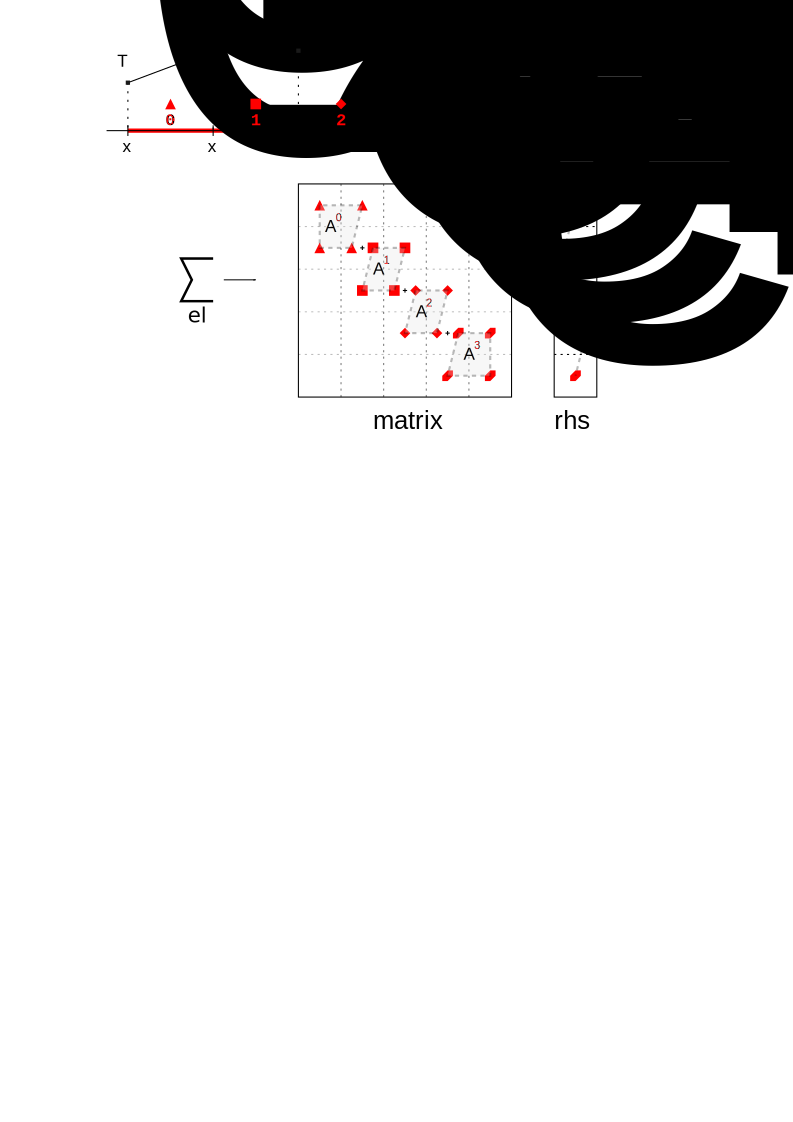
\includegraphics[width=8.5cm]{images/oneD/assembly}
\end{center}
The assembled matrix and rhs are then:
\[
\left(
\begin{array}{ccccc}
A_{11}^{{\color{red}\tt 1}} &  A_{12}^{{\color{red}\tt 1}} &0&0&0 \\ \\ 
A_{21}^{{\color{red}\tt 1}} &  A_{22}^{{\color{red} \tt 1}} \!+\! A_{11}^{{\color{red}\tt 2}}  & A_{12}^{{\color{red}\tt 2}}   &0&0 \\ \\
0& A_{21}^{{\color{red}\tt 2}} & A_{22}^{{\color{red} \tt 2}} \! +\! A_{11}^{{\color{red}\tt 3}}  & A_{12}^{{\color{red}\tt 3}}   & 0\\ \\
0&0& A_{21}^{{\color{red}\tt 3}}   & A_{22}^{{\color{red}\tt 3}} \! +\! A_{11}^{{\color{red}\tt 4}}   & A_{12}^{{\color{red}\tt 4}}  \\ \\
0&0&0& A_{21}^{{\color{red}\tt 4}}   & A_{22}^{{\color{red}\tt 4}} 
\end{array}
\right)
\left(
\begin{array}{c}
T_1 \\\\ T_2 \\\\ T_3 \\\\ T_4 \\\\ T_5
\end{array}
\right)
=
\left(
\begin{array}{c}
b_{1}^{{\color{red}\tt 1}} \\ \\
b_{2}^{{\color{red}\tt 1}} + b_{1}^{{\color{red}\tt 2}}\\ \\
b_{2}^{{\color{red}\tt 2}} + b_{1}^{{\color{red}\tt 3}}\\ \\
b_{2}^{{\color{red}\tt 3}} + b_{1}^{{\color{red}\tt 4}}\\ \\
b_{2}^{{\color{red}\tt 4}} 
\end{array}
\right)
\]
Ultimately the assembled matrix system also takes the form
\[
\left(
\begin{array}{ccccc}
A_{11} & A_{12} & 0& 0& 0\\ \\
A_{21} & A_{22} & A_{23}& 0 & 0\\\\
0 & A_{32} & A_{33}&  A_{34}  & 0\\\\
0&0&   A_{43} & A_{44}&  A_{45} \\\\
0&0&0   & A_{54}&  A_{55} \\\\
\end{array}
\right)
\left(
\begin{array}{c}
T_1 \\\\ T_2 \\\\ T_3 \\\\ T_4 \\\\ T_5
\end{array}
\right)
=
\left(
\begin{array}{c}
b_1\\\\
b_2\\\\
b_3\\\\
b_4\\\\
b_5
\end{array}
\right)
\]
and we see that it is sparse. Its sparsity structure is easy to derive: each row corresponds to a dof, 
and since nodes 1 and 2 'see' each other (they belong to the same element) there will be non-zero entries
in the first and second column. 
Likewise, node 2 'sees' node 1 (in other words, there is an edge linking nodes 1 and 2), itself, 
and node 3, so that there are non-zero entries in the second row at columns 1, 2, and 3.

Before we solve the system, we need to take care of boundary conditions.
Let us assume that we wish to fix the temperature at node 2, or in other words 
we wish to set 
\[
T_2 = T^{bc}
\]
This equation can be cast as
\[
\left(
\begin{array}{ccccc}
 0 & 1 & 0 & 0 & 0
\end{array}
\right)
\left(
\begin{array}{c}
T_1 \\ T_2 \\ T_3 \\ T_4 \\ T_5
\end{array}
\right)
=
\left(
\begin{array}{c}
0 \\
T^{bc} \\
0 \\
0 \\
0
\end{array}
\right)
\]

This replaces the second line in the previous matrix equation:
\[
\left(
\begin{array}{ccccc}
A_{11} & A_{12} & 0& 0& 0\\ \\
0 & 1 & 0 & 0 & 0 \\ \\
0 & A_{32} & A_{33}&  A_{34} & 0 \\\\
0&0&   A_{43} & A_{44}&  A_{45} \\\\
0&0&0   & A_{54}&  A_{55} \\\\
\end{array}
\right)
\left(
\begin{array}{c}
T_1 \\\\ T_2 \\\\ T_3 \\\\ T_4 \\\\ T_5
\end{array}
\right)
=
\left(
\begin{array}{c}
b_{1} \\ \\
T^{bc} \\ \\
b_{3}\\\\
b_{4}\\\\
b_{5}
\end{array}
\right)
\]
That's it, we have a linear system of equations which can be solved!






